\section{逆運動学及び順運動学の導出}

ここでは図\ref{fig:mecanum}に示すメカナムホイールロボットの運動学を導出する.

\begin{figure}[h]
  \centering
  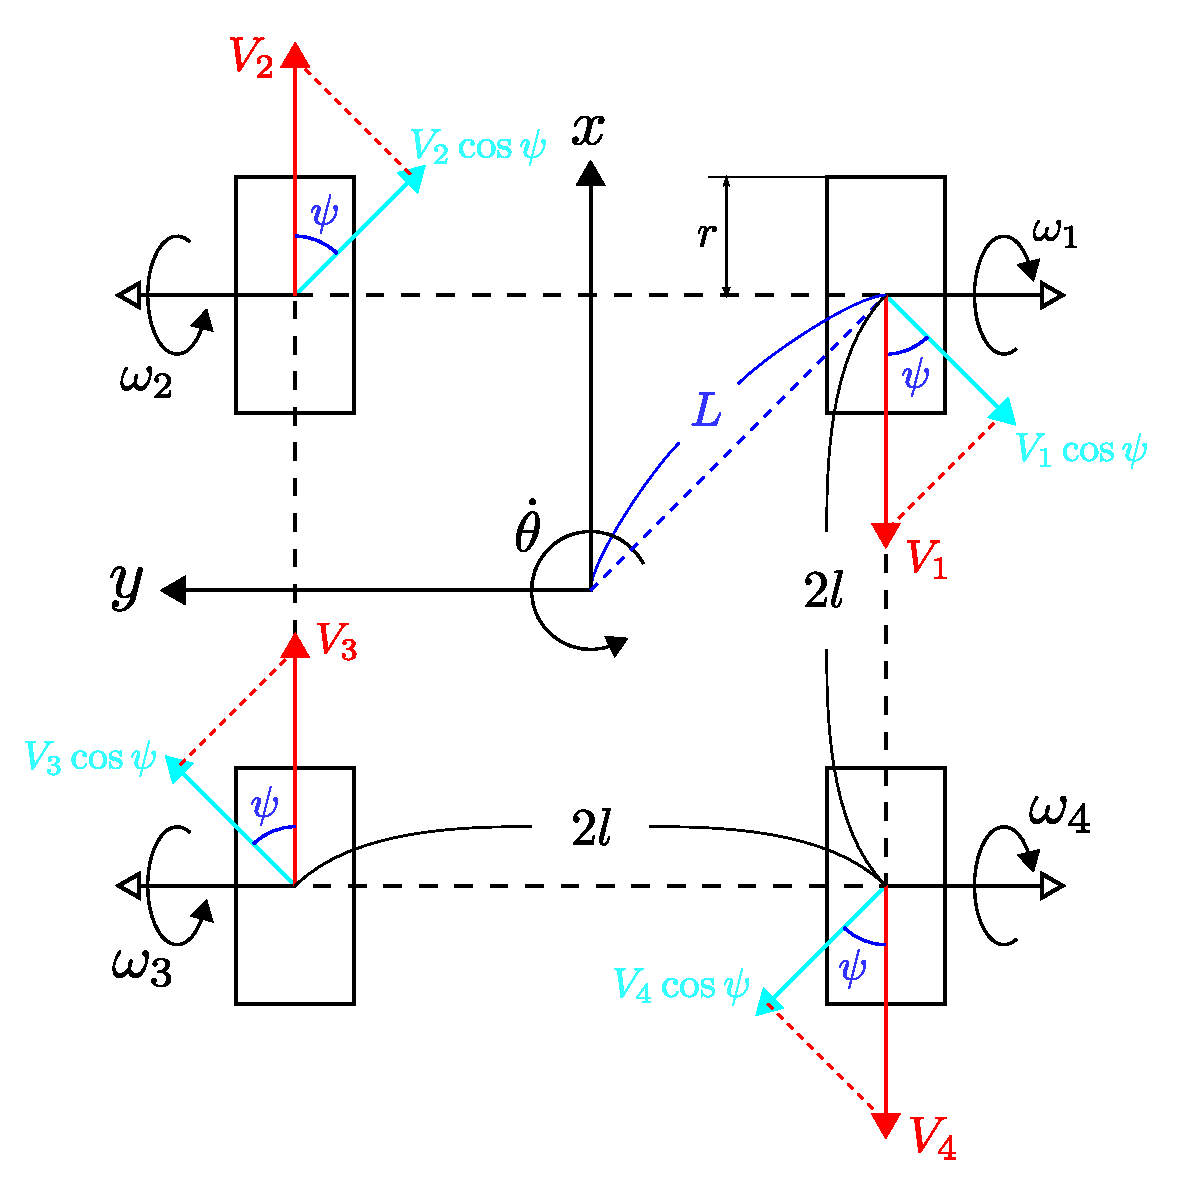
\includegraphics[width=120truemm, clip]{images/mecanum.pdf}
  \caption{4WD Mecanum Wheel}
  \label{fig:mecanum}
\end{figure}

\subsection{ロボットの各種パラメータ}

ロボット座標系は右手系座標系であり,原点はロボットの中心に固定されている.
$x$軸はロボットの前進方向に,$z$軸は鉛直上方向に設定されている.



ロボットは次のパラメータを持つ.

\begin{itemize}
  \item メカナムホイールの半径$r$
  \item ホイールのローラ角度$\psi =$\ang{45}
  \item ホイール間距離$2l$
  \item ロボット中心からホイールまでの距離$L = \sqrt{2}l$
  \item ホイール角速度$\omega_{i}$
  \item ホイールの周速度$V_{i} = r\omega_{i}$
  \item ロボットの速度の$x$軸方向成分$\dot{x}$
  \item ロボットの速度の$y$軸方向成分$\dot{y}$
  \item ロボットの角速度$\dot{\theta}$
\end{itemize}

メカナムホイールロボットはホイールが正方形の頂点上に配置されているタイプのものを考える.
また,ホイールのローラ角度は\ang{45}とする.

\subsection{逆運動学の導出}

メカナムホイールが回転すると,接地しているローラの軸方向に速度を発生させる.
その大きさはメカナムホイールの周速度$V_{i}$に$\cos{\psi}$を乗じたものになる.
ロボットの速度はホイールによってのみ発生することを考えると,式\ref{eq:inv1}が成り立つ.

\begin{subequations}
  \begin{empheq}[left=\empheqlbrace]{align}
    V_{1}\cos{\psi} &= - \dot{x}\cos{\psi} - \dot{y}\sin{\psi} - L\dot{\theta} \\
    V_{2}\cos{\psi} &=   \dot{x}\cos{\psi} - \dot{y}\sin{\psi} - L\dot{\theta} \\
    V_{3}\cos{\psi} &=   \dot{x}\cos{\psi} + \dot{y}\sin{\psi} - L\dot{\theta} \\
    V_{4}\cos{\psi} &= - \dot{x}\cos{\psi} + \dot{y}\sin{\psi} - L\dot{\theta}
  \end{empheq}
  \label{eq:inv1}
\end{subequations}

式\ref{eq:inv1}に$\psi =$\ang{45}を代入すると,式\ref{eq:inv2}が得られる.

\begin{subequations}
  \begin{empheq}[left=\empheqlbrace]{align}
    \frac{\sqrt{2}}{2} V_{1} &= - \frac{\sqrt{2}}{2}\dot{x} - \frac{\sqrt{2}}{2}\dot{y} - L\dot{\theta} \\
    \frac{\sqrt{2}}{2} V_{2} &= \frac{\sqrt{2}}{2}\dot{x} - \frac{\sqrt{2}}{2}\dot{y} - L\dot{\theta} \\
    \frac{\sqrt{2}}{2} V_{3} &= \frac{\sqrt{2}}{2}\dot{x} + \frac{\sqrt{2}}{2}\dot{y} - L\dot{\theta} \\
    \frac{\sqrt{2}}{2} V_{4} &= - \frac{\sqrt{2}}{2}\dot{x} + \frac{\sqrt{2}}{2}\dot{y} - L\dot{\theta}
  \end{empheq}
  \label{eq:inv2}
\end{subequations}

$\sqrt{2} L = \sqrt{2} \times \sqrt{l^2 + l^2} = 2l$であることを考慮して式\ref{eq:inv2}を変形すると,式\ref{eq:inv3}が得られる.

\begin{subequations}
  \begin{empheq}[left=\empheqlbrace]{align}
    V_{1} &= - \dot{x} - \dot{y} - 2l\dot{\theta} \\
    V_{2} &= \dot{x} - \dot{y} - 2l\dot{\theta} \\
    V_{3} &= \dot{x} + \dot{y} - 2l\dot{\theta} \\
    V_{4} &= - \dot{x} +\dot{y} - 2l\dot{\theta}
  \end{empheq}
  \label{eq:inv3}
\end{subequations}

式\ref{eq:inv3}を行列表示すると式\ref{eq:inv4}が得られる.

\begin{equation}
  \begin{pmatrix}
    V_{1} \\ V_{2} \\ V_{3} \\ V_{4}
  \end{pmatrix}
  =
  \begin{pmatrix}
     -1 & -1 & -2l \\
     1 & -1 & -2l \\
     1 & 1 & -2l \\
     -1 & 1 & -2l
  \end{pmatrix}
  \begin{pmatrix}
    \dot{x} \\
    \dot{y} \\
    \dot{\theta}
  \end{pmatrix}
  \label{eq:inv4}
\end{equation}

\subsection{順運動学の導出}

順運動学は,逆運動学の式を変形することで得られる.
今,式\ref{eq:inv4}の係数行列を$A$と置く.

\begin{equation*}
  \begin{pmatrix}
    V_{1} \\ V_{2} \\ V_{3} \\ V_{4}
  \end{pmatrix}
  =
  A
  \begin{pmatrix}
    \dot{x} \\
    \dot{y} \\
    \dot{\theta}
  \end{pmatrix}
  \label{eq:inv4}
\end{equation*}

順運動学を求めるには,$A$の逆行列$A^{-1}$を求めればよい.
しかし,$A$は正方行列ではないため,逆行列を持たない.
従って,疑似逆行列を用いる.
$A$の疑似逆行列$A^{+}$は$A^{+} = (A^{T}A)^{-1}A^{T}$で求められる.
これにより$A^{+}$が次のように求まる.

\begin{equation}
  A^{+} = \frac{1}{4}
  \begin{pmatrix}
    -1 & 1 & 1 & -1 \\
    -1 & -1 & 1 & 1 \\
    -\frac{1}{2l} & -\frac{1}{2l} & -\frac{1}{2l} & -\frac{1}{2l}
  \end{pmatrix}
\end{equation}

従って,式\ref{eq:forward}に示す順運動学が求まる.

\begin{equation}
  \begin{pmatrix}
    \dot{x} \\
    \dot{y} \\
    \dot{\theta}
  \end{pmatrix}
  =
  \begin{pmatrix}
    -1 & 1 & 1 & -1 \\
    -1 & -1 & 1 & 1 \\
    -\frac{1}{2l} & -\frac{1}{2l} & -\frac{1}{2l} & -\frac{1}{2l}
  \end{pmatrix}
  \begin{pmatrix}
    V_{1} \\ V_{2} \\ V_{3} \\ V_{4}
  \end{pmatrix}
  \label{eq:forward}
\end{equation}